\documentclass[a4paper]{report}

% Misc packages
\usepackage{amsmath}
\usepackage{graphicx}
\usepackage{multirow}

% Better font
\usepackage[protrusion=true,expansion=true]{microtype}
\usepackage[T1]{fontenc}
\usepackage{pxfonts}

% Clickable links
\usepackage{hyperref}
\hypersetup{
    colorlinks,
    citecolor=black,
    filecolor=black,
    linkcolor=black,
    urlcolor=black
}

% bibtex stuff
\usepackage{natbib}
\bibliographystyle{abbrvnat}

% Custom Commands
\newcommand{\degree}{\ensuremath{^\circ}}
\newcommand{\todo}{\textbf{TODO} }


\title{Literature Review of Point Cloud Compression}
\author{Keegan Smith\\ksmith@cs.uct.ac.za}

\begin{document}

\begin{titlepage}
\begin{center}


\includegraphics[width=100mm]{images/uct}\\
\ \\
\textsc{\Large
Department of Computer Science\\
\ \\
Honours Project Report\\
\ \\}

{\huge \bfseries
Intra-frame Compression of Molecular Dynamics Simulations of Water
\\}
\ \\
\ \\

\begin{center}
    \large Keegan Carruthers-Smith
    \\
    \small{ksmith@cs.uct.ac.za}
\end{center}

\vfill

{\large \today}

\end{center}
\end{titlepage}


\section*{Abstract}
Molecular dynamics (MD) simulations generate vast amounts of data. A typical
100-million atom MD simulation produces approximately 5 gigabytes of data per
frame consisting of atom types, coordinates and velocities.

The main contribution of the report is the specification of an MD compressor
which targets simulations with large amounts of water in it. Water is targeted
since many MD simulations contain significant amounts of water molecules. It
uses an approach based on predictive point cloud compressors, but with
predictors tailored towards models of water.

A point cloud is a collection of points in 3D space. The method improves on
existing point cloud compressors \citep{gumholdcomp,devillers2000gci} and MD
compressor \citep{omeltchenko2000sls} when applied to MD data with significant
amounts of water molecules.

There are six MD simulations the compression schemes are tested and compared
against. At $8$-bit quantisation the mean and average compression rate for
water compression is $19\%$. Gzip performs similarly at $8$-bit
quantisation. At $12$-bit quantisation the mean and average compression rate
for water compression is $31\%$. The next best scheme (gzip) has a mean and
average compression rate of $37\%$.

The report also presents techniques for compressing permutations. It presents
a technique which has a worst case performance that is approximately the lower
bound on the performance of a general permutation encoder. It also presents a
technique which probabilistically performs better than the lower bound.

\tableofcontents

\chapter{Introduction}

Molecular dynamics (MD) simulations generate vast amounts of data. A typical
$100$-million atom MD simulation produces approximately 5 gigabytes of data
per frame consisting of atom types, coordinates and velocities. This will
generate 17 terabytes of data a day if run for $35\,000$ steps with every
$10$\textsuperscript{th} frame being saved
\citep{omeltchenko2000sls}. Generating this much data makes compression
desirable useful for reducing storage space. A significant overhead in
simulations is also transmitting the data from the cluster which performs the
simulation to the researchers computer for analysis. Compression reduces the
transmission time.

Many MD simulations contain significant amounts of water molecules in
them. There are models on how water connect. Using this we have developed a
method which compresses MD simulations. It uses a connectivity-based point
cloud technique, but with predictors which are based on models of the
structure of water.

The method is compared against other point cloud compressors, as well as the
\citet{omeltchenko2000sls} MD compressor.

\todo explain intra-frame vs inter-frame compression
% An intra-frame compressor is one which compresses each frame of the
% compression independently of the other frames.

\paragraph{Research Question}

This report investigates the implementation and results of an intra-frame MD
data compressor which targets water. This compressor is considered successful if:

\begin{itemize}
  \item It can exploit water models.
  \item It can improve on other methods. Specifically point cloud compression
    methods.
  \item It can compress in an efficient manner? ($O(n^2)$ where $n$ is the
    number of atoms)
  \item It can decompress in an efficient manner? ($O(n)$)
\end{itemize}

Thus, the research question is whether it is possible to implement an
intra-frame compressor with the listed properties.


\paragraph{Outline}

In chapter two background information on MD file formats, compression, point
cloud compression and water models is discussed. Chapter three details the
design and implementation of the water compressor. Chapter four presents and
discusses the results from the implementation. Finally chapter five concludes
the report.



\chapter{Background}

This section starts by introducing the common file format used for storing MD
simulation data. It then moves on to the topic of compression which is
relevant to the rest of the report. This includes entropy encoding,
quantisation and predictive encoding. Point cloud compression algorithms are
then presented, as well as a taxonomy of point cloud compressors. The water
dimer model is also presented, with information on how it could be applied to
existing predictive point clouding techniques.

\section{Molecular Dynamics Format}
\label{sec:molec-dynam-form}

There are several Molecular Dynamics Simulations formats in use. The most
common format is the binary DCD file. DCD is also the default format used in
Visual Molecular Dynamics (VMD) \citep{vmd}. VMD is a molecular visualisation
program for displaying, animating, and analyzing molecular dynamics
simulations. VMD also relies on an accompanying PDB file to display the DCD
file.

There are multiple variations on the format of a DCD file, but they all store
the points in effectively the same way. VMD can handle two major variants,
CHARMm and X-PLOR, but VMD defaults to X-PLOR \citep{vmddcdformat}.

The DCD header contains at least the number of atoms and frames in the
simulations. Every atom is assigned an index $i$ between $0$ and $\#atoms -
1$. Each frame is then stored as an array of floating point values of size $3
\times \#atoms$. The location of atom $i$ is then stored at indicies $3 \times
i$ to $3 \times i + 2$ (storing the $x, y$ and $z$ coordinates). Atom $i$ will
always occur at index $3 \times i$ in every frame.

The DCD file only contains the positions of the atoms, with each item only
being identified by its index in a frame. Thus the DCD file does not contain
the atom's type. Instead this is contained in an accompanying PDB file.


\section{Compression}

Compression is the process of encoding information such that it uses less
storage than the unencoded form.

Compression algorithms can be either lossy or lossless. Lossless compression
algorithms do not ``lose'' any information during the encoding and decoding
process. An example of lossless compression is the gzip data compressor
\citep{gzip}. Lossy compression algorithms can ``lose'' information during the
encoding and decoding stages, but give approximations of the original
information. An example of a lossy compression algorithm is DivX for video
compression \citep{divx}.

\subsection{Entropy Encoders}

Entropy encoders attempt to optimally encode symbols as bits. A familiar
example of an entropy encoder is the Huffman Encoder. Given $n$ symbols
$\left\{x_1, \dots x_n \right\}$ each with corresponding probabilities
$\left\{p_1, \dots p_n \right\}$, Huffman Encoding assigns each $x_i$ a binary
codeword $c_i$ such that: \citep{huffman1952method}
\begin{enumerate}
  \item $p_i < p_j$ implies that $|c_j| \le |c_i|$ where $|c|$ is the length
    of the codeword $c$.
  \item There is no $c_i$ such that it is a prefix of $c_j$
\end{enumerate}

Huffman Encoding generates an optimal encoding which has the two listed
properties. Generation of the code takes $O(n \log n)$ time and $O(n)$ space.

Huffman Encoding has three main shortcomings. The first two problems are that
it requires the probabilities of each symbol and it needs to store the mapping
for decoding. Both of these problems are remedied by Adaptive Huffman Encoders
\citep{drozdek,vitter1987}. These start with every symbol having equal
probability, and then proceed to efficiently update the probabilities as each
symbol is encoded.

The final shortcoming is that each symbol is mapped to a prefix-free binary
codeword. The amount of wastage caused by this could be as much as one bit per
symbol. Arithmetic Coding is an alternative approach which can encode a symbol
as a fractional amount of bits \citep{drozdek}. Arithmetic Coding achieves
this by encoding the entire message as a rational number in $[0,1)$. Each
  symbol $x_i$ is assigned a disjoint subrange of $[0,1)$ with size $p_i$.

Encoding is done by adjusting the lower and upper bound of what the encoded
rational number will be. Initially the lower bound is $l=0$ and the upper
bound is $u=1$. Then when encoding a symbol $x_i$ which is assigned the range
$[a,b)$ the bounds are adjusted to
\begin{align*}
  l' & = l + a * (u-l) \\
  u' & = l + b * (u-l)
\end{align*}

Arithmetic coding has a similiar shortcoming to Huffman Encoding, in that it
requires the probabilities of each symbol and needs to store the
probabilities. This can be overcome by using an Adaptive Arithmetic Encoder
\citep{drozdek}. Initially all symbols have equal probability and as each
symbol is encoded the ranges are updated.

Implementations of Arithmetic Encoding usually separate out the model and the
encoder. The model keeps track of what the probabilities of each symbol are,
while the encoder writes out the rational. The encoder does not store the full
rational, but instead writes out each bit of the binary decimal expansion. It
can write the bit when the lower bound is such that the bit will not
change. Encoding and decoding is $O(1)$.

The static model is just a look-up table of the probabilities, so can be
implemented to be $O(1)$. The adaptive model uses Fenwick trees
\citep{fenwick1994new} to update and query frequencies in $O(\log n)$ time.


\subsection{Quantisation}

\todo Diagram

The data encoded by the algorithms in this report are usually stored as
floating point values. A process called \emph{quantisation} reduces the
precision of a floating point value to an integer value
\citep{ag-racm-03}. \emph{Dequantisation} converts the integer value back into
an approximation of the original floating point value. Quantisation is
inherently lossy.

If the bounds of the data are known, then the range of the data can be
uniformly divided up. Then each sample is assigned the index of the range it
falls into \citep{drozdek}. This is called \emph{linear quantisation}. By
storing the bounds and the number of buckets the range is divided up into,
original values can be approximated.

Linear quantisation of point coordinates involves quantising each coordinate
separately and uniformly in Cartesian space. This can be visualised as
creating an evenly-spaced grid over the dimensions of the space, and snapping
the points to the closest grid point.

There are more complex methods reviewed by \citet{ag-racm-03}. These lie
outside the scope of the report.


\subsection{Predictive Coding}

Predictive coders exploit inter-correlation of data to achieve compression
\citep{drozdek}. If the data in the format is point positions then
neighbouring points are inter-correlated. So using the encoded neighbouring
points, a predictive encoder would predict where the point is. The encoder
would then encode the difference between the points location and its predicted
location (known as the residual).

Linear quantisation preserves the inter-correlation of the points. So if the
points are quantised first, then the residuals can be encoded using an entropy
encoder such as an arithmetic coder. If the predictor is accurate, the
residuals will mostly be small values. So the probability of the small values
will be high, leading to good compression.

Using the residuals and the predictions the decoder can reconstruct the point
locations.


\section{Point Cloud Compression}

A point cloud is a collection of point locations in 3D space. Research has
concentrated on point clouds of surfaces since point clouds are usually
generated from 3D scans of object surfaces. A surface is the ``skin'' of an
object, i.e. the boundary of a solid object.

Every point cloud compressor in this report (except \citet{chen2005lcp}) first
quantise the points using linear quantisation. In all the point cloud
compressors reviewed, this is the only lossy step. \citet{chen2005lcp} gets
around quantisation by treating the 32-bit floating point numbers as 32-bit
integers.

\citet{gumholdcomp} create a tree of the points that exploit the knowledge that
the points lie on a surface. They do not, however, use predictors which
exploit this. \citet{merrycomp} extend this by using predictors which do
exploit the rectilinear nature of surface scans.

\citet{omeltchenko2000sls} compress point clouds from molecular dynamics
simulations. To exploit the density of the point clouds, a space filling curve
is created along the quantised positions. A space filling curve is one that
touches every point in a discrete space. The space filling curve used by
\citet{omeltchenko2000sls} is based on indexing the cells created by an octree
division. Then by encoding the difference between successive indicies which
contain points, they generate consistently small differences leading to good
compression rates.

\citet{devillers2000gci} compress meshes of 3D models. A mesh is a collection
of vertices, edges and faces defining a 3D object. The method they use only
considers point locations, so it can be used for point cloud
compression. Their method exploits a property of kd-trees, instead of general
geometric properties.


\subsection{Predictors}

A rooted spanning tree of the point is used in both \citet{gumholdcomp} and
\citet{merrycomp}. The creation of the spanning tree depends on what
predictor(s) are used and will be described in \ref{sec:serialisation}. For
each point $v$ in the spanning tree let $v'$ be the point's parent and $v''$
be the point's grandparent.

\citet{gumholdcomp} lets the user choose between two predictors. The first is
a \emph{constant} predictor where $v$ is predicted to be at $v'$. The second
is a \emph{linear} predictor where $v$ is predicted to be at $v' + (v' -
v'')$. So either $v$ is in the same place as its parent, or it is along the
straight line $(v', v'')$ with distance $|v'-v''|$ away from its parent.

\citet{merrycomp} use the same predictors as \citet{gumholdcomp} but with two
additional predictors, the \emph{left} and \emph{right} predictors. The
surface normal\footnote{A surface normal at a point $v$ is the normal of the
  plane tangent to the surface at $v$.} $n_v$ at $v$ is heuristically
determined from $v, v'', v'$ and $n_{v'}$ (where $n_{v'}$ is the surface
normal at $v'$). From this they determine what left and right are by using the
plane determined by $n_{v'}, v'$ and $v''$. Another difference to
\citet{gumholdcomp} is that instead of letting the user choose the
predictor used, the best predictor is picked for each point. This requires the
predictor used at each point to be encoded, which is discussed next.


\subsection{Serialisation}
\label{sec:serialisation}

Unlike meshes, point clouds have no connectivity information. So there is no
obvious order to serialize the vertex information (generally residuals). By
creating a spanning tree of the points, serialisation can occur by walking the
graph. The tree also needs to be encoded so decoding can recover the tree to
do the walk.

\citet{gumholdcomp} create a rooted spanning tree of the points. The points
are first sorted along the $x, y$ or $z$ axis. The tree is then greedily
created by picking the first point as a root and then adding each successive
point to the vertex which minimises the residual. The tree is then serialized
by entropy encoding the out degree of each vertex in breadth-first order.

\citet{merrycomp} also create a rooted spanning tree of the points, but in a
way that favours ``long runs'' of the forward predictor. They need to encode
the predictor used at each point, so encoding the tree as \citet{gumholdcomp}
did will not work. Instead the tree is serialized by entropy coding the
predictor used in depth-first order. By favouring long runs of the forward
predictor they get better compression ratios of the encoding of the tree. To
create the spanning tree, they first create a graph of the points where every
edge with length less than $L$ is added. $L$ is the length of the longest edge
in the minimum spanning tree of the complete graph of the points. The spanning
tree is then created similarly to Prim's algorithm \citep[p.\ 457]{sedgewick},
but instead using a metric\footnote{A metric is a way to calculate the
  distance between vertices.} that favours recently considered vertices and
ones predicted well by the forward predictor.

\citet{chen2005lcp} uses a spanning tree with differential coding on the
weights. So the point cloud is encoded as a tree, with edge weights being the
difference vectors between points. They show that there exists a spanning tree
which minimises the number of pairwise different edge weights, but also show
that this is NP-Hard. They do, however, give an approximate algorithm which
uses clustering and minimum spanning trees. The tree is serialized in a simple
breadth-first order, recording the number of children for each node and the
edge weights for each child.


\section{Decoding}

When decoding the data, we may present to the user intermediate
representations of the final decompressed data as we process it. This is a
desirable property if the user can use the intermediate representations while
(s)he waits for the final representation to be
transferred/decompressed. Depending on whether we can do this or not gives us
another way to classify encoders.

\paragraph{Progressive Encoder}
A progressive encoder is one that starts out streaming a coarse representation
of a point cloud. It then streams out refinements. This is useful for
transmitting the data over a network, as users can almost instantaneously see
a coarse representation. This is then followed by more and more refinements
over time as they arrive.

The use case of MD simulations require the whole file (or frame) to be
decompressed. So progressive encoders have no advantage, and are judged purely
on how well they compress the data.

\citet{devillers2000gci} provide an example of a progressive coder. The method
is best explained in one dimension first. If you know the total number of
points in $[a, b]$ (say $x$ points) and the number of points in $[a, (a+b)/2]$
(say $y$ points) then the number of points in $[(a+b)/2+1, b]$ is $x - y$ . By
sending out counts of deeper and deeper levels in breadth first order they
progressively get a better representation. Encoding this with arithmetic
coding gives us the desired compression ratios. To extend to 3 dimensions one
uses a process similiar to creating a kd-tree: at each step subdivide along a
different dimension.

\paragraph{Single-Rate Encoding}
A single-rate encoder is one which requires the whole stream to be available
before the data can be decompressed. \citet{omeltchenko2000sls},
\citet{gumholdcomp} and \citet{merrycomp} are all single-rate encoders. In
general single-rate encoders imply better compression.


\section{Modelling Water}
\label{sec:modelling-water}

\begin{figure}[h]
\centering
\resizebox{0.75\textwidth}{!}{
  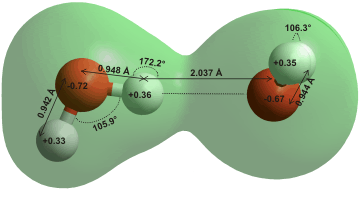
\includegraphics{images/h402}
}
\caption{The most energetically favourable water dimer calculated from first
  principles. \citep{watermolecule}}
\label{fig:dimer}
\end{figure}

\todo Redraw figure \ref{fig:dimer-angle}
\begin{figure}[h]
\centering
\resizebox{0.5\textwidth}{!}{
  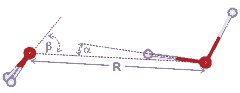
\includegraphics{images/dimr}
}
\caption{Water dimer angles. $R = 2.976\AA, \alpha = 6 \pm 20\degree, \beta =
  57 \pm 10\degree$. \citep{watermolecule}}
\label{fig:dimer-angle}
\end{figure}

The previously discussed predictors work well in the setting of general point
clouds, but in a point cloud consisting of water molecules we can create
predictors tailored towards water.

A water dimer is two water molecules loosely bonded by a hydrogen atom. This
is the simplest model for hydrogen bonding in water, and as such has been
extensively studied.

The oxygen which is loosely bonded to the hydrogen is expected to be
$2.976\AA$ away from the other oxygen. It is also expected that the vector
created by the O-H bond to be roughly in line with the vector of the loose O-H
bond \citep{watermolecule}. See Figure \ref{fig:dimer} and Figure
\ref{fig:dimer-angle}.

\subsection{Using the Model in Point Cloud Compressors}

\citet{omeltchenko2000sls} only exploit the fact that there may be many dense
clusters in MD simulations. It is more general than water compression, and how
to modify it to use the relative layouts of the water molecules is unclear.

The predictors of \citet{merrycomp} and \citet{gumholdcomp} do not exploit the
layout of water molecules. Using water dimer model prediction can be done
given the positions of a water molecules atoms. The creation of the spanning
tree would be different, since we know the expected degree of the verticies is
at most two.

\begin{table}[t]
\centering
\resizebox{\textwidth}{!}{
\begin{tabular}{||l|c|c||}
  \hline
  \emph{Attribute/Method} & \citet{omeltchenko2000sls} & \citet{gumholdcomp} \\

  \hline

  \emph{Structure} & MD Simulation & Surface \\

  \emph{Progressive} & Single-rate & Single-rate \\

  \emph{Quantisation} & Yes & Yes \\

  \emph{Connectivity} & Space Filling Curve & Spanning Tree \\

  \emph{Exploits} & Dense/regular clusters & Regularity of scans \\

  \emph{Scope} & Global & Local \\

  \emph{Topology} & Geometry & Both \\

  \hline
  \hline

  \emph{Attribute/Method} & \citet{chen2005lcp} & \citet{devillers2000gci} \\

  \hline

  \emph{Structure} & 3D Model & Mesh \\

  \emph{Progressive} & Single-rate & Progressive \\

  \emph{Quantisation} & No & Yes \\

  \emph{Connectivity} & Spanning Tree & kd-trees \\

  \emph{Exploits} & Differential Coding & kd-tree properties \\

  \emph{Scope} & Global & Global \\

  \emph{Topology} & Connectivity & Neither \\

  \hline
  \hline

  \emph{Attribute/Method} & \citet{merrycomp} & \\

  \hline

  \emph{Structure} & Surface & \\

  \emph{Progressive} & Single-rate & \\

  \emph{Quantisation} & Yes & \\

  \emph{Connectivity} & Spanning Tree & \\

  \emph{Exploits} & Rectilinear scans & \\

  \emph{Scope} & Local & \\

  \emph{Topology} & Both & \\

  \hline
\end{tabular}
}
\caption{Taxonomy of the different methods.}\label{tab:taxonomy}
\end{table}


\section{Taxonomy of Techniques}

Refer to Figure \ref{tab:taxonomy} for an overview of the categorisations of
the different papers. There are two underlying philosophies which the
compression algorithms exploit: \emph{scope} and \emph{topology}.

\emph{Scope} is whether the algorithm is exploiting \emph{global} or
\emph{local} properties of the points. \citet{merrycomp} uses a local scope
since it exploits nearby points to predict the location of the current
point. \citet{chen2005lcp} uses a global scope, since it is trying to minimise
a global property of the spanning tree.

\emph{Topology} is whether the algorithm is trying to exploit connectivity or
geometric information. \citet{gumholdcomp} exploit both, but the geometry more
since it uses a predictor to predict the location based on other points
location. \citet{chen2005lcp} just tries to choose the best possible spanning
tree, so they exploit connectivity of points.

The other properties listed in the taxonomy are \emph{structure},
\emph{progressive}, \emph{quantisation}, \emph{connectivity} and
\emph{exploits}.

\begin{itemize}
\item \emph{Structure} is what type of point cloud the compressor targeting.

\item \emph{Progressive} is whether the compressor is a single-rate encoder or
  progressive encoder.

\item \emph{Quantisation} is whether the compressor applies quantisation
  before compression.

\item \emph{Connectivity} is how relationships between points are derived or
  modelled.

\item \emph{Exploits} is what the compressor is targeting for good
  compression.
\end{itemize}


\section{Summary}

The water dimer model gives a good predictor for exploiting the local
structure of water molecules. So, using a predictive point cloud encoder
similiar to \citet{merrycomp} and \citet{gumholdcomp} should result in good
compression of water molecules than previous methods.

Compressing the other atoms will require a more general technique. Using the
best point cloud compressor on the other atoms combined with the water
prediction scheme should result in better compression.


\chapter{Design and Implementation}

This chapter outlines the design and implementation of our compressor and
decompressor. The compression techniques investigated only cover intra-frame
compression, where compression occurs per frame independently of the other
frames. Reference implementations of other schemes, inter-frame compression as
well as visualisation, were implemented as independent subsystems, as such the
design needs to take into account these uses. Components outside of the scope
of intra-frame compression will not be covered in detail.

The main contribution of this report is a predictive encoder targeting water
molecules. The compressor is referred to as the Water Compressor.

\section{Overview}

Compression is done on the DCD/PDB format, which is a format for storing MD
simulations. DCD files are explained in Section \ref{sec:molec-dynam-form}.

A high-level overview of how data flows in the compressors is illustrated by
the following: \todo replace with pretty picture similiar to the FBI
fingerprint compression paper

\[ DCDFile \to Atoms \to QuantisedAtoms \to Compressor \]

The decompressor works in the reverse direction:

\[ Decompressor \to QuantisedAtoms \to DCDFile \]

The decompressed DCD files are an approximation due to quantisation. Excluding
this quantisation step, the schemes are lossless. Note that each step in the
compression phase has auxillary information. The auxillary information is
required for reconstruction.

Reference implementations of \citet{devillers2000gci}, \citet{gumholdcomp} and
\citet{omeltchenko2000sls} are also implemented. These use the I/O and
quantisation components. Julian Kenwood implemented
\citet{omeltchenko2000sls}, while Keegan Carruthers-Smith implemented
\citet{devillers2000gci} and \citet{gumholdcomp}. Visualisation uses the I/O
and quantisation components as well and was implemented by Min-Young Wu.


\subsection{Dependencies}

All development was done on Linux, but no Linux or POSIX specific APIs where
used. The implementations should be cross platform, but this has not been
tested.

\paragraph{C++}
A language which produces fast and optimised code is necessary since run time
is important in compression. All of the authors are competent in C++, thus all
the components are written in C++. Development was done with GCC 4.x.

\paragraph{ANN}
This is a library for approximate nearest neighbor searching. It is used to
speed up graph creation where locality of points is important, \citep{ann}.

\paragraph{VMD DCD Loader Plugin}
This plugin is used to read and write DCD files, \citep{vmd}.


\section{Components}
\label{sec:components}

A component-based approach was used to design the compressor and decompressor,
since the algorithm can be broken up into distinct steps.

\todo picture showing components and who did what

The components are as follows:

\paragraph{Simulation I/O}

These components handle I/O to and from the simulation data files. The VMD DCD
loader plugin is used to load and write the DCD files. A PDB reader for
determining what each atom is in the DCD file is also implemented. DCD is used
since it is the prevalent format for storing simulation data, and it is well
supported in VMD.


\paragraph{Arithmetic Coder}

The water compression scheme as well as the point cloud schemes use arithmetic
encoding of the residuals and tree. The range of the residuals in the
predictive schemes as well as the number of different residuals is not known
beforehand. As such the usual model used in arithmetic encoding does not
fit.

For the model we use a novel approach which is based the on adaptive
arithmetic model. It uses similiar to the technique by
\citet{cormack1984algorithms} used in Adaptive Huffman Encoding. The adaptive
model initially only has one symbol meaning ``new'' symbol. When encoding if
there is a new symbol, the ``new'' symbols is encoded followed by a raw
representation of the new symbol. By using a prefix tree and a modification of
Fenwick trees \citep{fenwick1994new}, insertion of new symbols into the model
is $O(n \log n)$ where $n$ is the number of seen symbols.

The encoder by \citet{omeltchenko2000sls} does not make use of an Arithmetic
Coder, instead it uses its own entropy coder. Every other encoder uses the
arithmetic encoder.


\paragraph{Quantiser}

The quantiser is responsible for quantising and dequantising a frame. The
quantiser takes in as input a number $b$. The quantiser quantises each
dimension independently using linear quantisation. The number of cells it
divides each dimension into is $2^b$. So after quantisation each coordinate
becomes a $b$-bit integer.

Linear quantisation is chosen since the water compressor (as well as the other
predictive compressor) requires the locality of the points to be
preserved. Quantisation is also necessary since small differences in
predictive residuals should be treated as the same for better entropy
encoding.

Converting the floating point values to integers introduces error. But for the
predictive schemes to be effective it is necessary. This is the only step
which is lossy. In the literature if the only lossy step is quantisation, the
algorithm is still referred to as lossless.


\paragraph{Permutations}

When decompressing we need to recover the atoms in the same order they are
listed in the original DCD file. The water compressor as well as the other
predictive point cloud schemes do not recover the original order. How
permutations are encoded is explained in Section \ref{sec:compr-perm}.


\paragraph{Compressors}

The compressor component is different for each compressor. It implements the
encoding and decoding of the quantised frames. The intra-frame compressors
which are implemented are the water compressor and reference implementations
of \citet{omeltchenko2000sls}, \citet{gumholdcomp} and
\citet{devillers2000gci}.


\paragraph{Verifiers}

Verifiers are for testing whether a compression scheme is working. Given a DCD
file and a decompressed DCD file, if the files match when quantised then the
compressor is considered functional. There is the possibility of floating
point error causing a mismatch when the files are in fact equivalent. This
happens infrequently, so the frames which do not match can be inspected
manually to see if they are the same.


\section{Compressing Permutations}
\label{sec:compr-perm}

Compression algorithms explored in this report do not necessarily preserve the
order of the points when decompressed. For example in \citet{devillers2000gci}
\[ (1, 2), (1, 3), (0, 0), (2, 3), (2, 2), (0, 2), (1, 1) \]
when decompressed becomes
\[ (0, 0), (1, 1), (0, 2), (1, 2), (1, 3), (2, 2), (2, 3) \]

When decompressing we need to recover the original order of the points, since
the index of a point indicates which atom it is in the DCD file format.

We experimented with five different types of permutation compressors. Each
permutation compressor takes in a permutation of $[0,1,\dots,N-1]$ and encodes
it to the file. Let the permutation be $[P_0, P_1, \dots P_{N-1}]$. The
decompressor then recovers the permutation.

\paragraph{Null}
Null does not write anything to the file. The decompressor just outputs the
order permutation $[0,1,\dots,N-1]$. A compressor which uses the null
compressor does not preserve the order. As such the null is only used for
reference.

\paragraph{Na\"{\i}ve}
Na\"{\i}ve writes the permutation list straight to the file. Each index is
stored as an unsigned $32$-bit integer. Every other permutation compressor
should do better than this.

\paragraph{Delta}
Delta transforms the permutation into a list $L$, where $L_0 = P_0$ and $L_i =
P_i - P_{i-1}$ for $0 < i < N$. Arithmetic encoding is then done on $L$, which
is then written to file.

Decompression gets back the list $L$. Since $P_0 = L_0$ and $P_i = L_i +
P_{i-1}$ for $0 < i < N$ we can recover the original permutation. Since each
$P_i$ depends only on previous $i$'s, calculating $P_i$ in increasing order of
$i$ will recover $P$.

\paragraph{Interframe}
Interframe tries to exploit the correlation of the permutation lists between
frames. Interframe transforms the permutation $P$ into a list $L$. Let $P'$ be
the permutation from the previous frame. If it is the first frame, let $P' =
[0,1,\dots,N-1]$. Then $L_i = P_i - P'_i$ for $0 \le i < N$. Arithmetic
encoding is used on $L$ and it is then written to file.

Decompression recovers the list $L$. Since $P_i = L_i + P'_i$, $P$ can be
recovered. Note that this method requires frames to be decompressed in order.

Using this scheme causes an intra-frame encoder to become interframe. The
objective of this report is constructing an intra-frame compressor, but this
is still experimented with since the permutation encoding ended up being a
significant portion of the compressed file. The results indicated that this
scheme did not perform best, as such the best encoders remain intra-frame.

\paragraph{Optimal}
Each $P_i$ occurs only once, so the frequency of each $P_i$ is known per
encoding. Optimal uses a static arithmetic coder with a frequency of one for
each $P_i$.

A static arithmetic encoder model uses a Fenwick Tree \citep{fenwick1994new}
to update the symbol table after each encoding. This takes $O(\log(N))$ per
update. In the optimal permutation compressor we can get this down to $O(1)$
by using the fact that we only ever encode each $P_i$ once.

To encode a symbol $i$ the arithmetic encoder requires $S_{tot}$, $S_i$ and
$S_{i-1}$. $S_{tot}$ is the sum of all the frequencies. $S_i$ is the sum of
the frequencies for all the symbols less than or equal to $i$. Since the
frequency of each index is one, $S_i = i$ and $S_{tot}$ is the number of
permutations left. We need a way to map permutation indicies to symbols which
is quick to update once an index has been encoded. The following algorithm is
used:

\begin{verbatim}
init(permutation):
  number_of_symbols = permutation.size
  for i in 0, 1, ..., permutation.size - 1:
    index_to_symbol[i] = i
    symbol_to_index[i] = i
\end{verbatim}

\begin{verbatim}
pop_index(index):
  number_of_symbols--

  symbol = index_to_symbol[index]
  index2 = symbol_to_index[number_of_symbols]

  index_to_symbol[index2] = symbol;
  symbol_to_index[symbol] = index2;

  return symbol;
\end{verbatim}

\begin{verbatim}
pop_symbol(symbol):
  index = symbol_to_index[symbol]
  pop_index(index)
  return index
\end{verbatim}

To encode $P_i$, we encode $pop\_index(P_i)$. To decode, we return
$pop\_symbol(val)$ where $val$ is a value returned from the arithmetic
decoder.

\todo an example of this in action

The optimal permutation encoder is optimal in the worst case. If we have $M$
indicies left to encode, each unseen index has probability $\frac{1}{M}$ of
occurring and every seen index has probability $0$ of occurring. So for each
$i$ we have that $S_{tot}=M, S_i = i, S_{i-1} = i-1$. This gives a probability
of $\frac{i-(i-1)}{M} = \frac{1}{M}$.

If there are $M$ indicies left, the lower-bound on the number of bits to
encode an index is $\log_2(M)$. So if $P$ has $N$ indicies a lower-bound on
the number of bits to encode $P$ is
\begin{equation}
  \displaystyle\sum^{N}_{i=1} \log_2(i)
  \label{eq:optimal-lowerbound}
\end{equation}
Each index can fit into $\lceil\log_2(N)\rceil$ bits, so this is used as an
effective upper-bound. See Table \ref{tab:optimal-lowerbound} for values of
Equation (\ref{eq:optimal-lowerbound}) in bytes. Notice how as the size of the
permutation increases, the gains made by the optimal scheme decrease.


\begin{table}
  \center
  \resizebox{\textwidth}{!}{
  \begin{tabular}{|l|rrrrrr|}
    \hline
    \emph{Permutation Size} & $1$ & $2$ & $10$ & $1000$ & $10\,000$ &
    $100\,000$ \\
    \hline
    \emph{Lower-Bound} & $0.00$ & $0.12$ & $2.72$ & $1066.17$ & $14807.26$ &
    $189588.02$ \\
    \emph{Effective Upper-Bound} & $0.00$ & $0.25$ & $5.00$ & $1250.00$ &
    $17500.00$ & $212500.00$ \\
    \emph{Percentage Gain} & $0.00$ & $33.33$ & $29.47$ & $7.94$ & $8.33$ &
    $5.70$ \\
    \hline
  \end{tabular}
  }
  \caption{Number of bytes needed for storing permutations of different
    sizes. See Equation (\ref{eq:optimal-lowerbound}) for the lower bound. The
    effective upper-bound is
    $\lceil\log_2(N)\rceil/8$.} \label{tab:optimal-lowerbound}
\end{table}

The optimal encoder is optimal since on its worst permutation it does better
than any other encoder, but most of the encoders have a low probability of
encountering a bad permutation. There may also be inter-correlation amongst
subsets of the permutation. So probabilistically the \emph{delta} encoder will
do better than the \emph{optimal} encoder. If the permutations between frames
are correlated, then the \emph{interframe} encoder will likely do better than
the \emph{optimal} encoder.


\section{Water Compressor}

This section details the algorithm of the water compressor and is the main
contribution of this report. The encoder is implemented as a compressor
component and uses the components detailed in the Section
\ref{sec:components}.

The compressor processes each quantised frame in order. This encoder is a
predictive intra-frame encoder, and as such only compresses using information
contained in the frame.

The algorithm is similiar to the predictive point cloud compressors of
\citet{gumholdcomp} and \citet{merrycomp}. The following is a high level
overview of the algorithm:

\begin{verbatim}
CompressFrame(list_of_atoms_in_frame, arithmetic_encoder):
  list_of_water_molecules = FindWater(list_of_atoms_in_frame)
  list_of_other_atoms = FindNonWater(list_of_atoms_in_frame)
  compress(list_of_other_atoms, arithmetic_encoder)
  water_graph = CreateGraph(list_of_water_molecules)
  spanning_tree = CreateSpanningTree(water_graph)
  TreeSerialise(spanning_tree, arithmetic_encoder)
\end{verbatim}

\noindent Similarly decompression uses this algorithm:

\begin{verbatim}
DecompressFrame(arithmetic_decoder):
  list_of_other_atoms = decompress(arithmetic_decoder)
  list_of_water_atoms = TreeDeserialise(arithmetic_decoder)
  return list_of_other_atoms + list_of_water_atoms
\end{verbatim}

The compression of non-water atoms simply involves writing out the quantised
positions of the frame. This is done for two reasons: the permutation
information is stored for ``free'' and the number of other atoms is expected
to be small.

An explanation of each step follows, along with motivation of why each step is
done.


\subsection{Finding Water Molecules}

The PDB file associated with a DCD file contains information on which atoms a
given atom is bonded to. Using the PDB file the encoder finds all oxygen atoms
which are bonded to two hydrogen atoms. This section was implemented in the
Simulation I/O component.

The implementation returns two lists: a list of water molecule indicies and a
list of other atom indicies. Every water molecule is specified using the
indicies in the frame of its corresponding oxygen and hydrogen atoms. Every
index which is not in a water molecule is stored in the second list.

The split between water molecules and other atoms is done so that compression
of water molecules and the other atoms can be done using different
encoders. The water compression predictors target water atoms, so a more
general compression method is used on the other atoms.


\subsection{Water Predictors}
\label{sec:water-predictors}

The predictors are based on the models of water dimers explained in the
background chapter. There are three predictors used, a constant predictor and
two hydrogen predictors.

When prediction is applied a tree is made of the water molecules. Then each
molecule is predicted from its parent in the tree. Let $O, H_1, H_2$ be the
predictions for where the water molecule will be and let $O', H'_1, H'_2$ be
the water molecules parent.

\paragraph{Constant Predictor}
The constant predictor predicts $O$ to be at $O'$. This predictor is included
since occasionally the hydrogen bond is broken (molecule information remains
static from the start of the simulation). If the bonds are broken the hydrogen
predictors are far less accurate than the constant predictor.

\paragraph{Hydrogen Predictor}
The hydrogen predictor predicts along $O'-H'_1$ or $O'-H'_2$. We simplify the
model in Figure \ref{fig:dimer-angle} and assume $\alpha$ is $0\degree$. Then
$O$ is predicted to be at $O' + 2.976\frac{O'-H'_i}{|O'-H'_i|}$.

In all three prediction schemes $H_1$ and $H_2$ are predicted to be at
$O$. This is since their is a large variability in $\beta$ in Figure
\ref{fig:dimer-angle}.


\subsection{Creating the Water Graph}

Creating the spanning tree is $O(E \log E)$, where $E$ is the number of edges
in the graph. When creating the spanning tree, each molecule's predictions are
compared to all of its neighbours. If the graph created is the complete graph,
$E$ is $O(N^2)$, where $N$ is the number of water molecules. However, this is
too inefficient for large scale simulations.

So the purpose of graph creation is to efficiently minimise the degree of the
verticies (and hence $E$), while maintaining the neighbours which predict well
against the predictors.

The neighbours which predict well are related to the spatial locality of the
oxygens. So the approximation used is to add edges between all molecule pairs
where the oxygens are within $3\AA$. The degree of a vertex is then a small
number (typically less than five) and the number of edges created is usually
$O(N)$.

The na\"{i}ve implementation of graph creation would compare each molecule
against every other, yielding a $O(N^2)$ algorithm. Again this is too
slow. Instead a kd-tree \citep{cormen2001introduction} is used to create the
graph. A kd-tree is a space-partitioning data structure which allows quick
queries based on locality of points. The kd-tree is populated with the oxygen
positions. Then using ANN's approximate fixed radius search one can find all
other oxygens within approximately $3\AA$. Creating the graph requires $O(N
\log N)$ time. The fixed radius search takes approximately $O(\log N)$
time. The search is done per molecule, so the overall time complexity for
graph creation is $O(N \log N)$. The algorithm is as follows:

\begin{verbatim}
createGraph(list_of_water_molecules):
  graph = graph of water molecules
  kdtree = KDTree(list_of_water_molecules.O_pos)
  for cur_mol in list_of_water_molecules:
    radius = 3 angstroms
    for mol in kdtree.fixed_radius_search(cur_mol.O_pos, radius):
      graph.addEdge(cur_mol, mol)
  return graph
\end{verbatim}



\subsection{Creating the Spanning Tree}

The order in which the points are serialised, and which predictor is used for
each point is not obvious from the graph created in the previous section. A
directed tree is created from the graph since each molecule is predicted by
one other molecule. The edge $O' \to O$ indicates that $O$ is predicted using
the position of $O'$.

The graph is not necessarily connected, so a spanning tree is created for each
component. A root vertex is arbitrarily selected. Then each tree in the forest
is connected to the root with the constant predictor. Each edge $O' \to O$ is
labelled with what predictor is used to predict $O$ from $O'$.

For each component a root is arbitrarily picked. The tree is then created by
using a modification of Dijkstra's shortest path algorithm
\citep{dijkstra1959note}. The priority queue stores potential edges, and sorts
by the residual from the prediction. When a potential edge $O' \to O$ is
removed from the queue, it is added to the spanning tree if $O$ is not already
in it. The algorithm is illustrated by the following:

\begin{verbatim}
create_spanning_component(graph, tree, component_root, root):
  priority_queue q
  q.add(0, component_root -> root, constant)
  while q not empty:
    residual, v' -> v, p = q.pop()

    if v not in tree:
      tree add edge v' -> v with predictor p

    predictions = { constant_predictor(p),
                    h1_predictor(p),
                    h2_predictor(p) }

    for u in graph[v].children:
      if u in tree:
        continue

      residual, predictor = smallest_residual(u, predictions)

      q.add(residual, v -> u, predictor)
\end{verbatim}

This algorithm is $O(E \log E)$ since for every edge in the graph, a potential
edge is added to the queue. In the implementation an optimisations is used
which reduces the complexity to approximately $O(N \log E)$. In this
optimisation the smallest seen residuals is kept for each molecule. Then a
potential edge $v \to u$ is only added if the residual is less than the
current smallest residual for $u$.


\subsection{Tree Serialisation}

This stage encodes the predictions and spanning tree. The predictions are
encoded in breadth first order. The spanning tree is also encoded since it is
required to reconstruct what each molecule is predicted from. The BFS then
starts at the root of the spanning tree and for each molecule in the BFS the
following happens:

\begin{verbatim}
process(O' -> O, predictor):
  prediction  = prediction(O', predictor)
  O_residual  = water_molecule.oxygen - prediction
  H1_residual = water_molecule.hydrogen1 - water_molecule.oxygen
  H2_residual = water_molecule.hydrogen2 - water_molecule.oxygen

  residual_encoder.encode({ O_residual, H1_residual, H2_residual })
  permutation_encoder.encode(water_molecule.index)

  for pred, child in O.children:
    tree_encoder.encode(pred)
    bfs_queue.push(O -> child, pred)
  tree_encoder.encode(sentinel)
\end{verbatim}

The root does not have a predictor, so by default the constant predictor will
predict the position to be $(0,0,0)$.


\paragraph{Deserialisation}

The tree deserialisation is the reverse of the serialisation. It populates a
quantised frame with the following algorithm:

\begin{verbatim}
q = queue()
q.push(NULL, constant_predictor)

while q not empty:
  parent, predictor = q.pop()

  prediction  = predict(parent, predictor)
  O_position  = residual_decoder.decode() + prediction
  H1_residual = residual_decoder.decode() + O_position
  H2_residual = residual_decoder.decode() + O_position

  index = permutation_decoder.decode()
  water_molecules[index].oxygen    = O_position
  water_molecules[index].hydrogen1 = H1_position
  water_molecules[index].hydrogen2 = H2_position
\end{verbatim}

Since this is done for each atom once per frame, decoding takes $O(N)$ time.


\section{Conclusion}

\todo


\chapter{Results}

\todo Need to give section on how often constant vs hydrogen prediction is
done.

Testing was done on an Intel Quad Core 2.66GHz machine with 4GB of RAM. Each
encoding scheme was tested against 6 DCD files at $8$-bit and $12$-bit
quantisation.

Each encoding scheme was tested with all the permutation encoders listed in
Section \ref{sec:compr-perm}. When showing the result of an encoding scheme,
the \emph{null} permutation encoder is shown. What is also shown is the best
performing permutation encoder, excluding \emph{null}, on the run.

Two additional compressors are also tested. These are straight quantisation
(referred to as \emph{quant}) and quantisation followed by the data compressor
gzip (referred to as \emph{gzip}).

The encoder by \citet{gumholdcomp} has two possible predictors to use, the
\emph{constant} predictor and the \emph{linear} predictor. The results here
indicate only the use of the \emph{constant} predictor since it always did
better than the \emph{linear} predictor. This is due to a non-linear
relationship between points in molecular dynamics data, unlike rectilinear
scans.

\section{Datasets}

\begin{table}[t]
\resizebox{\textwidth}{!}{
\begin{tabular}{|lrrrrl|}
\hline

\emph{Name} & \emph{Size} & \emph{Atoms} & \emph{Frames} & \emph{\% Water} &
\emph{Comment} \\

\hline

smallwater & $0.8$ & $699$ & $100$ & $100\%$ & Small water box \\

rabies & $11$ & $464\,099$ & $2$ & $68\%$ & Rabies virus with two areas of water \\

hiv & $38$ & $16\,470$ & $200$ & $93\%$ & HIV in water \\

hotwater & $222$ & $96\,603$ & $200$ & $100\%$ & Water at $1\,000\degree$C \\

water & $244$ & $96\,603$ & $220$ & $100\%$ & Water at room temperature \\

mscl & $382$ & $111\,016$ & $300$ & $61\%$ & Mechanosensitive Channel \\

\hline
\end{tabular}
}
\caption{Description of DCD files used in compression tests. Size is in
  megabytes.} \label{tab:testdata}
\end{table}

Six different DCD files were used in the experiments. Every DCD file excluding
MSCL was generated by Julian Kenwood using the Nanoscale Molecular Dynamics
(NAMD). A summary of each file is given in Table \ref{tab:testdata}.

\begin{itemize}
\item{\textbf{Small Water}} is a simulation containing $233$ water
  molecules. The simulation is run at room temperature. The file contains
  every frame of the simulation.
\item{\textbf{Water}} is a simulation of $32\,301$ water molecules. The
  simulation is run at room temperature ($25\degree$C). The file contains
  every $50^{th}$ frame of simulation.
\item{\textbf{Hot Water}} is the same simulation as \emph{Water}, but at
  $1\,000\degree$C.
\item{\textbf{HIV}} is a simulation of a part of the Human Immunodeficiency
  Virus(HIV) surrounded by water. It is simulated at room temperature
  ($25\degree$C). The file contains every $50^{th}$ frame of simulation.
\item{\textbf{Rabies}} is a simulation of the rabies virus. The simulation is
  run at room temperature. The file contains every frame of the simulation.
\item{\textbf{MSCL}} is a simulation of a protein which is separating two
  volumes of water. The protein is called Mechanosensitive Channels. This DCD
  file was donated by Dr.~James Gain. The output rate is unknown, but
  inspection of the simulation in VMD indicates erratic movement of the atoms.
\end{itemize}

The two most important attributes of the simulation is the temperature and the
number of atoms. The number of atoms affect the run time of the schemes per
frame. The temperature affects the accuracy of the water model. The higher the
temperature, the worse the expected performance of the water compressor is.

\section{Compression Results}

For each run the compression size and time where recorded. The decompression
time where also tested, but are not listed. This is since every schemes
excluding \citet{devillers2000gci} has linear decompression
complexity. \citet{devillers2000gci} has $O(n \log n)$ decompression
complexity, which is the same as the compression complexity, so times are
similiar. The results for $8$-bit and $12$-bit compression are presented
separately.

\subsection{8-bit Quantisation}

\begin{table}[h]
\centering
\resizebox{\textwidth}{!}{
\begin{tabular}{|lr|rrr|rr|rr|rr|}
  \hline
  \multirow{2}{*}{\textbf{DCD}} & \multirow{2}{*}{\textbf{atoms}} & \multirow{2}{*}{\textbf{quant}} & \multirow{2}{*}{\textbf{gzip}} & \multirow{2}{*}{\textbf{omel}} & \multicolumn{2}{|c|}{\textbf{gumhold}} & \multicolumn{2}{|c|}{\textbf{dg}} & \multicolumn{2}{|c|}{\textbf{watercomp}} \\
   &  &  &  &  & \emph{null} & \emph{best} & \emph{null} & \emph{best} & \emph{null} & \emph{best} \\

  \hline

  smallwater & $699$ & $25.35$ & $\textbf{\emph{12.30}}$ & $30.00$ & $19.34$ & $27.66$ & $21.74$ & $26.45$ & $19.87$ & $22.97$ \\

  water & $96\,603$ & $25.00$ & $21.47$ & $27.72$ & $\emph{11.20}$ & $26.00$ & $12.86$ & $24.10$ & $11.77$ & $\textbf{17.05}$ \\

  hotwater & $96\,603$ & $25.00$ & $19.08$ & $26.43$ & $\emph{10.48}$ & $25.56$ & $11.31$ & $22.67$ & $11.35$ & $\textbf{16.65}$ \\

  rabies & $464\,099$ & $25.00$ & $\textbf{13.86}$ & $27.78$ & $\emph{9.28}$ & $25.69$ & $10.17$ & $22.05$ & $15.01$ & $19.44$ \\

  hiv & $16\,470$ & $25.02$ & $24.12$ & $27.96$ & $\emph{13.89}$ & $26.98$ & $15.81$ & $26.67$ & $14.69$ & $\textbf{18.74}$ \\

  mscl & $111\,016$ & $25.00$ & $20.17$ & $27.69$ & $\emph{11.22}$ & $25.89$ & $12.41$ & $23.39$ & $16.88$ & $\textbf{20.05}$ \\

  \hline
\end{tabular}
}
\caption{Compression rates at $8$-bit quantisation. The best ratio is
  bolded. The \emph{null} permutation values are also included, but are not
  considered since they do not restore the correct order of
  points. \emph{Best} is the permutation encoder which did the best out of
  \emph{delta}, \emph{interframe}, \emph{na\"{i}ve} and \emph{optimal}.}
\label{tab:res8}
\end{table}

See Table \ref{tab:res8} for the $8$-bit compression ratios. The results
indicate that in general that the water compression scheme performs best. If
the ordering of the points is not important, the best scheme is
\citet{gumholdcomp} (see column gumhold null). The water compression scheme
without ordering information has ratios which are very close to gumhold
null. So without ordering information water compression still performs well.

See Figure \ref{fig:speed8} for the $8$-bit compression speeds. This graph
indicates that the water compression algorithm can perform relatively worse in
terms of speed. This is due to the $O(e \log e)$ spanning tree creation
step. All other algorithms are $O(n \log n)$ where $n$ is usually an order of
magnitude less than $e$. The algorithm is still efficient though since it is
sub $O(n^2)$.

The worst running time the water compression algorithm had was $693$ seconds
on \emph{water}. This further indicates that it may be worse relatively, but
still acceptable. The algorithm performs best in terms of compression ratio,
so the trade-off is valid.

\begin{figure}[h]
\centering
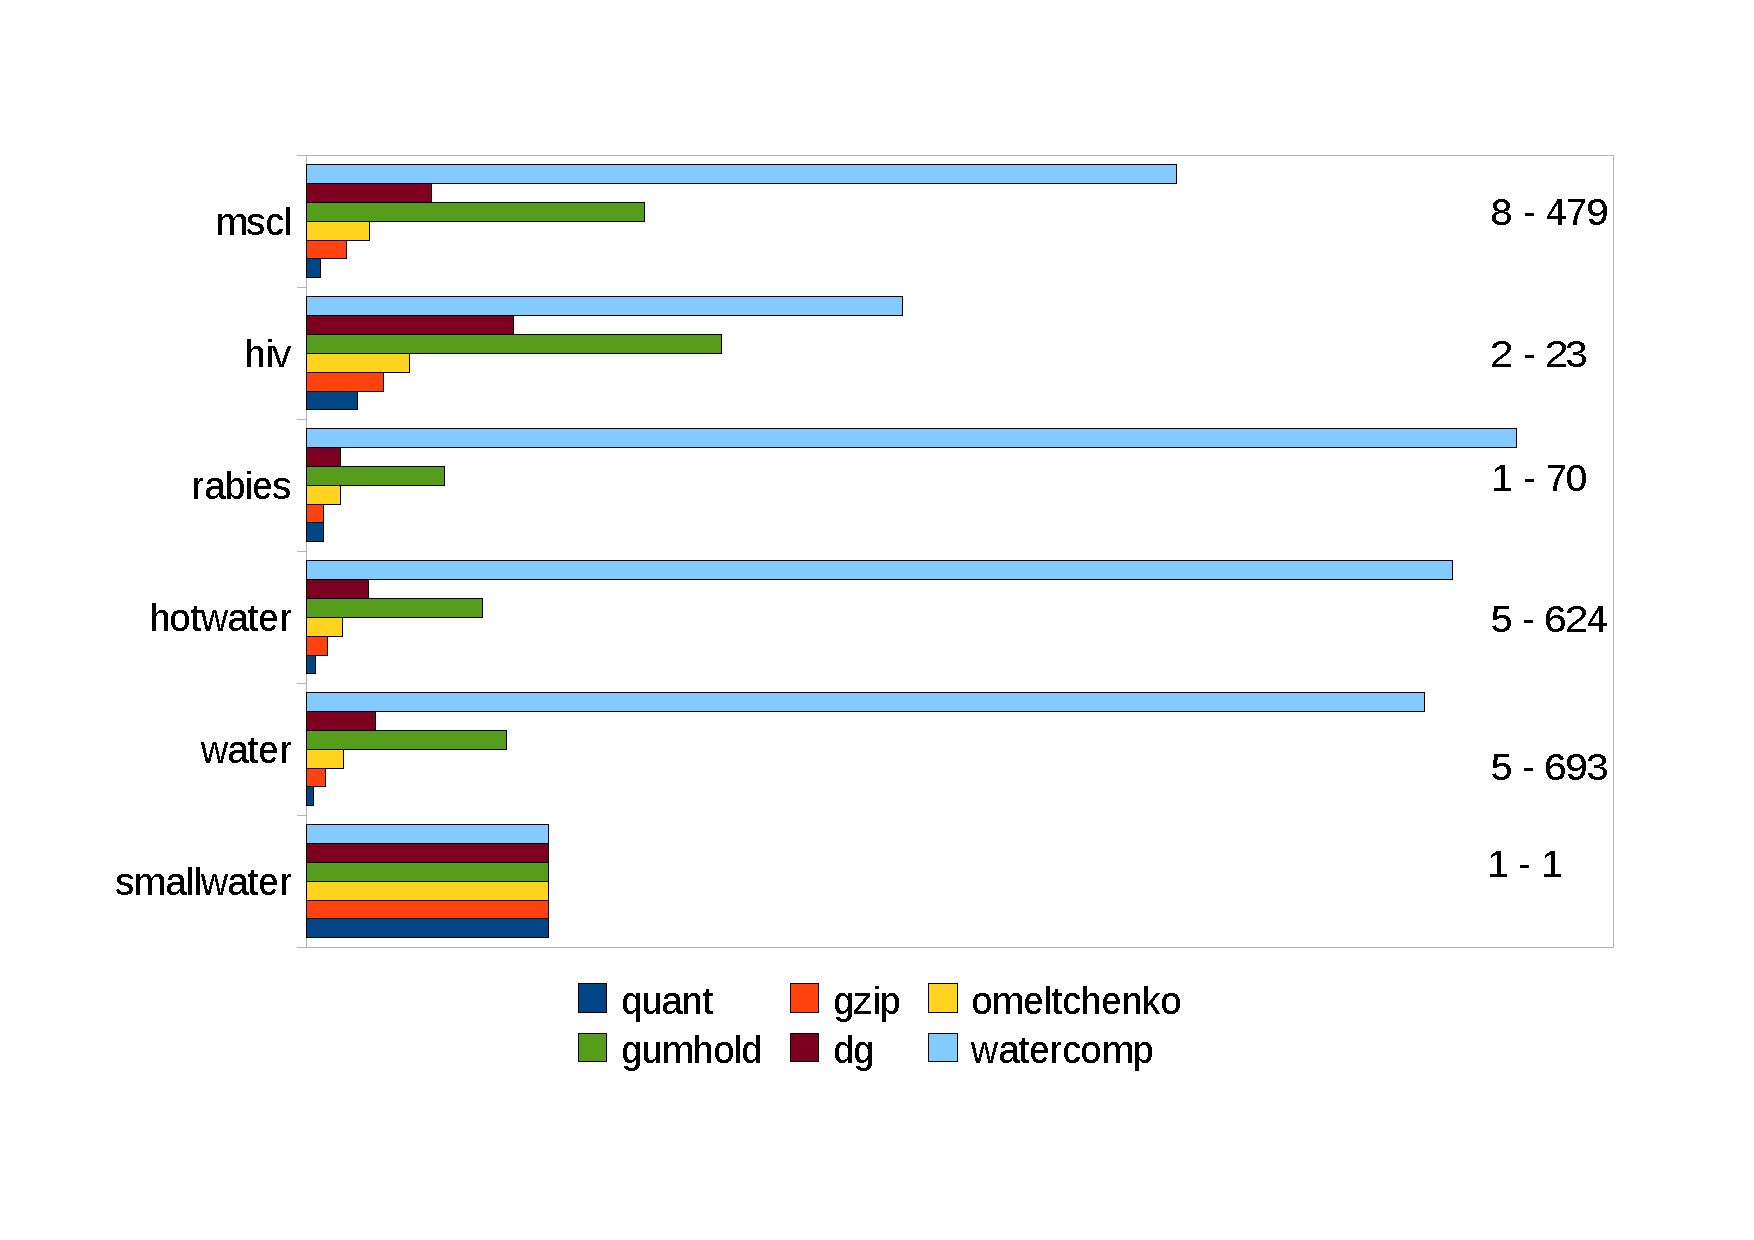
\includegraphics{images/speed8}
\caption{The relative time taken for each compression scheme at $8$-bit quantisation.}
\label{fig:speed8}
\end{figure}


\subsection{12-bit Quantisation}

\begin{table}[h]
\centering
\resizebox{\textwidth}{!}{
\begin{tabular}{|lr|rrr|rr|rr|rr|}
  \hline
  \multirow{2}{*}{\textbf{DCD}} & \multirow{2}{*}{\textbf{atoms}} & \multirow{2}{*}{\textbf{quant}} & \multirow{2}{*}{\textbf{gzip}} & \multirow{2}{*}{\textbf{omel}} & \multicolumn{2}{|c|}{\textbf{gumhold}} & \multicolumn{2}{|c|}{\textbf{dg}} & \multicolumn{2}{|c|}{\textbf{watercomp}} \\
   &  &  &  &  & \emph{null} & \emph{best} & \emph{null} & \emph{best} & \emph{null} & \emph{best} \\

  \hline

  smallwater & $699$ & $37.83$ & $37.39$ & $43.86$ & $\emph{32.75}$ & $41.07$ & $34.99$ & $39.69$ & $34.11$ & $\textbf{36.61}$ \\

  water & $96\,603$ & $37.50$ & $37.26$ & $40.23$ & $\emph{23.62}$ & $38.40$ & $26.50$ & $37.74$ & $23.97$ & $\textbf{29.21}$ \\

  hotwater & $96\,603$ & $37.50$ & $36.82$ & $38.92$ & $\emph{22.95}$ & $38.03$ & $25.19$ & $36.54$ & $23.37$ & $\textbf{28.70}$ \\

  rabies & $464\,099$ & $37.50$ & $32.92$ & $40.27$ & $\emph{21.64}$ & $38.00$ & $24.12$ & $36.00$ & $27.16$ & $\textbf{31.59}$ \\

  hiv & $16\,470$ & $37.51$ & $37.52$ & $40.51$ & $\emph{26.30}$ & $39.39$ & $29.25$ & $40.10$ & $27.28$ & $\textbf{31.33}$ \\

  mscl & $111\,016$ & $37.50$ & $37.19$ & $40.19$ & $\emph{23.63}$ & $38.22$ & $26.06$ & $37.04$ & $29.29$ & $\textbf{32.47}$ \\

  \hline
\end{tabular}
} \caption{Compression rates at $12$-bit quantisation. The best ratio is
  bolded. The \emph{null} permutation values are also included, but are not
  considered since they do not restore the correct order of
  points. \emph{Best} is the permutation encoder which did the best out of
  \emph{delta}, \emph{interframe}, \emph{na\"{i}ve} and \emph{optimal}.}
\label{tab:res12}
\end{table}

See Table \ref{tab:res12} for the $12$-bit compression ratios. The results
indicate that the water compression scheme performs best for all the DCD
files. If the ordering of the points is not important, the best scheme is
\citet{gumholdcomp} (see column gumhold null).

Similiar to the $8$-bit results, the water compression scheme without ordering
information has ratios which are very close to gumhold null. The cases where
it does not are the rabies and mscl. Both of these do not contain as much
water as the good result, so the non-water points compression make up the
difference. Without ordering information water compression still performs
well.

See Figure \ref{fig:speed12} for the $12$-bit compression speeds. This graph
is nearly identical to the $8$-bit graph (\ref{fig:speed8}). The difference is
that the water compression scheme has run times closer in speed to the other
schemes. This is since the run-time is dominated by the spanning tree
creation, which is not affected by the granularity of the quantisation.

The worst increase in run time for the water compression scheme from $8$-bit
to $16$-bit is on MSCL. It increased by $21$ seconds, from $479$ seconds to
$500$ seconds. The increase in time is probably accountable to the increased
number of different residuals due to the higher precision. If the number of
residuals increase, the performance of the arithmetic encoder decreases (but
the decrease is logarithmic, which can be ignored).


\begin{figure}[h]
\centering
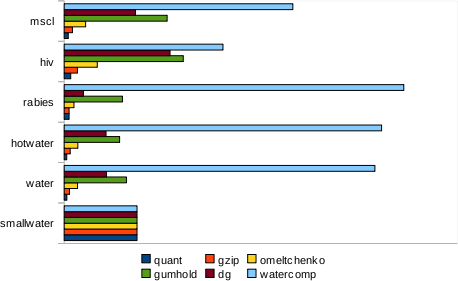
\includegraphics{images/speed12}
\caption{The relative time taken for each compression scheme at $12$-bit quantisation.}
\label{fig:speed12}
\end{figure}


\section{Permutation Results}

Studying the differences between the null and best columns in Tables
\ref{tab:res8} and \ref{tab:res12} indicate that a significant portion of the
compression is lost due to the encoding of the permutation. In some cases
encoding the permutation causes the scheme to perform worse than just
quantising the file.

Figure \ref{fig:perm} shows the relative performance of each permutation
encoder with the water compressor at $12$-bit quantisation. The best
permutation encoder is the \emph{delta} encoder. The pathological cases which
cause poor performance are unlikely, which is why the \emph{delta} encoder
performed well.

The most stable encoder is the \emph{optimal} encoder. This is since the size
of the encoding is related to the size of the permutation (see Equation
(\ref{eq:optimal-lowerbound}).

\begin{figure}[h]
\centering
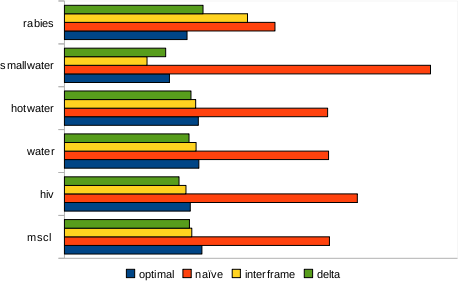
\includegraphics{images/perm}
\caption{The relative performance of the permutation encoders on different DCD
  files. The encoder used is the water compressor at $12$-bit quantisation.}
\label{fig:perm}
\end{figure}


\section{Summary}
\label{sec:summary}

From the results it can be seen that the water compression scheme performs
best. If the order of the points does not need to be recovered then the
encoder by \citet{gumholdcomp} performs best. However water compression
performs nearly as well as \citet{gumholdcomp}.

The speed of the water compressor can be up to three times slower than the
next slowest scheme. However the water compressor performs best, and the
actual elapsed time was at most $11$ minutes.

The permutation information requires a significant portion of the compressed
file. In some of the references scheme it caused the compression to be worse
than simply quantising the file. The best permutation encoder was the
\emph{delta} encoder, while the most stable was the \emph{optimal} encoder.



\chapter{Conclusion}

The water compression scheme compresses better than existing other point cloud
compressors (Section \ref{sec:summary}). This is since it exploits the
water-dimer model (Section \ref{sec:modelling-water} and
\ref{sec:water-predictors}). At $8$-bit quantisation the mean and average
compression rate for water compression is $19\%$. At $12$-bit quantisation the
mean and average compression rate for water compression is $31\%$.

The permutation information required a significant portion of the compressed
file. A permutation encoder called \emph{optimal} was shown to take
approximately $\sum^{N}_{i=1} \log_2(i)$ where $N$ is the size of the
permutation (Section \ref{sec:compr-perm}). The formula is a lower bound on
the worst performance of a permutation encoder.

Probabilistically the worst case permutation will not occur when using the
\emph{delta} encoder. The results indicate that this encoder performs best.

The complexity of encoding in the water compression scheme is $O(n + n \log n
+ e \log e + n) = O(e \log e)$ where $e = O(n^2)$ and $n$ is the number of
water molecules. Empirically and due to the theoretical models of water, $e$
is typically less than $5 \times n$, and so $e = O(n)$. So the encoding time
is $O(n \log n)$. The decoding time is $O(n)$.


\section{Future Work}

\paragraph{Parallelism}

Intra-frame compressors work independently of each frame. This allows
parallising over frames.

\paragraph{General Molecular Dynamics Predictors}

Running an approximate simulation and using the positions it obtains as
predictors should give good general predictors. This also does not need to
store the permutation information.

\paragraph{Better joining of components in spanning tree}

The water compressor implementation joins up the components by adding an edge
to a route. This is currently done in a na\"{i}ve way. Possible ways include
using a MST of the components or encoding the components separate to the
errors. Adapting \citet{chen2005lcp} is another possibility.

\paragraph{Point Cloud Compressor which preserve ordering}

A large portion of the compressed data involved storing the permutation. A
point cloud compressor which preserves the ordering is likely to perform very
well at MD compression.

\nocite{*}
\bibliography{report_keegan}

\end{document}

% LocalWords:  oxygens Deserialisation BFS MSCL intra DCD
